Another algorithm for meta reinforcement learning is evolved policy gradient (EPG)\cite{epg}. Unlike meta gradient algorithm which focuses on learning the return function, EPG aims to learn a surrogate loss function $L_\phi = L_{\phi + \sigma\epsilon_i}$, which is parameterized by parameter $\phi$ along with a small Gaussian noise $\epsilon_i \sim \mathcal{N}(0, \mathbf{I})$ as perturbed terms.

\par
EPG contains an inner loop and an outer loop during its execution. In inner loop, the algorithm functions as normal policy gradient algorithm that tries to update policy parameter $\theta$ according to the following formula:

\[\theta^* = \argmin_\theta\EX_{\tau\thicksim\mathcal{M},\pi_\theta}[L_\phi(\pi_\theta,\tau)]\]

where $\theta^*$ is the updated parameter $\theta$, $\mathcal{M}$ is a sampled markov decision process, $\tau$ is an episode of $\mathcal{M}$ with horizon $\textit{H}$. The objective of the inner loop is to minimize the loss function $L_\phi$. In outer loop, EPG adopts evolutionary strategies because there is no explicit way to write down a differentiable equation between the return and the loss function. The loss function parameter $\phi$ is updated as shown below:

\[\phi^* = \argmax_\phi\EX_{\mathcal{M}\thicksim p(\mathcal{M})}\EX_{\tau\thicksim\mathcal{M},\pi_{\theta^*}}[R_\tau]\]

where $p(\mathcal{M})$ is a distribution over MDPs, $\pi_{\theta^*}$ is the agent's policy trained with the loss function $L_\phi$ and $R_\tau = \sum_{t=0}^{H}\gamma^t{r_t}$ is the discounted episodic return of $\tau$. The goal of the outer loop is to achieve high expected returns in the MDP distribution.

\par
Pseudocode of EPG algorithm is shown in Fig. \ref{epg}. The algorithm works as follows: Because of adoption of evolutionary strategies, $\textit{W}$ workers will work in the inner loop. Then, at the beginning of each epoch in the outer loop, $\textit{V}$ multivariate normal vectors $\epsilon_v \in \mathcal{N}(0,\mathbf{I})$ of the same dimension as the loss function parameter $\phi$ are generated and assigned to $\textit{V}$ loss functions $L_v = L_{\phi+\delta\epsilon_v}$ respectively, with $\textit{v}$ being the $\textit{v}$-th generated perturbed parameters. Then $\textit{W}$ workers are divided into $\textit{V}$ groups and each group obtain the $\textit{v}$-th loss function.
\begin{figure}[H]
	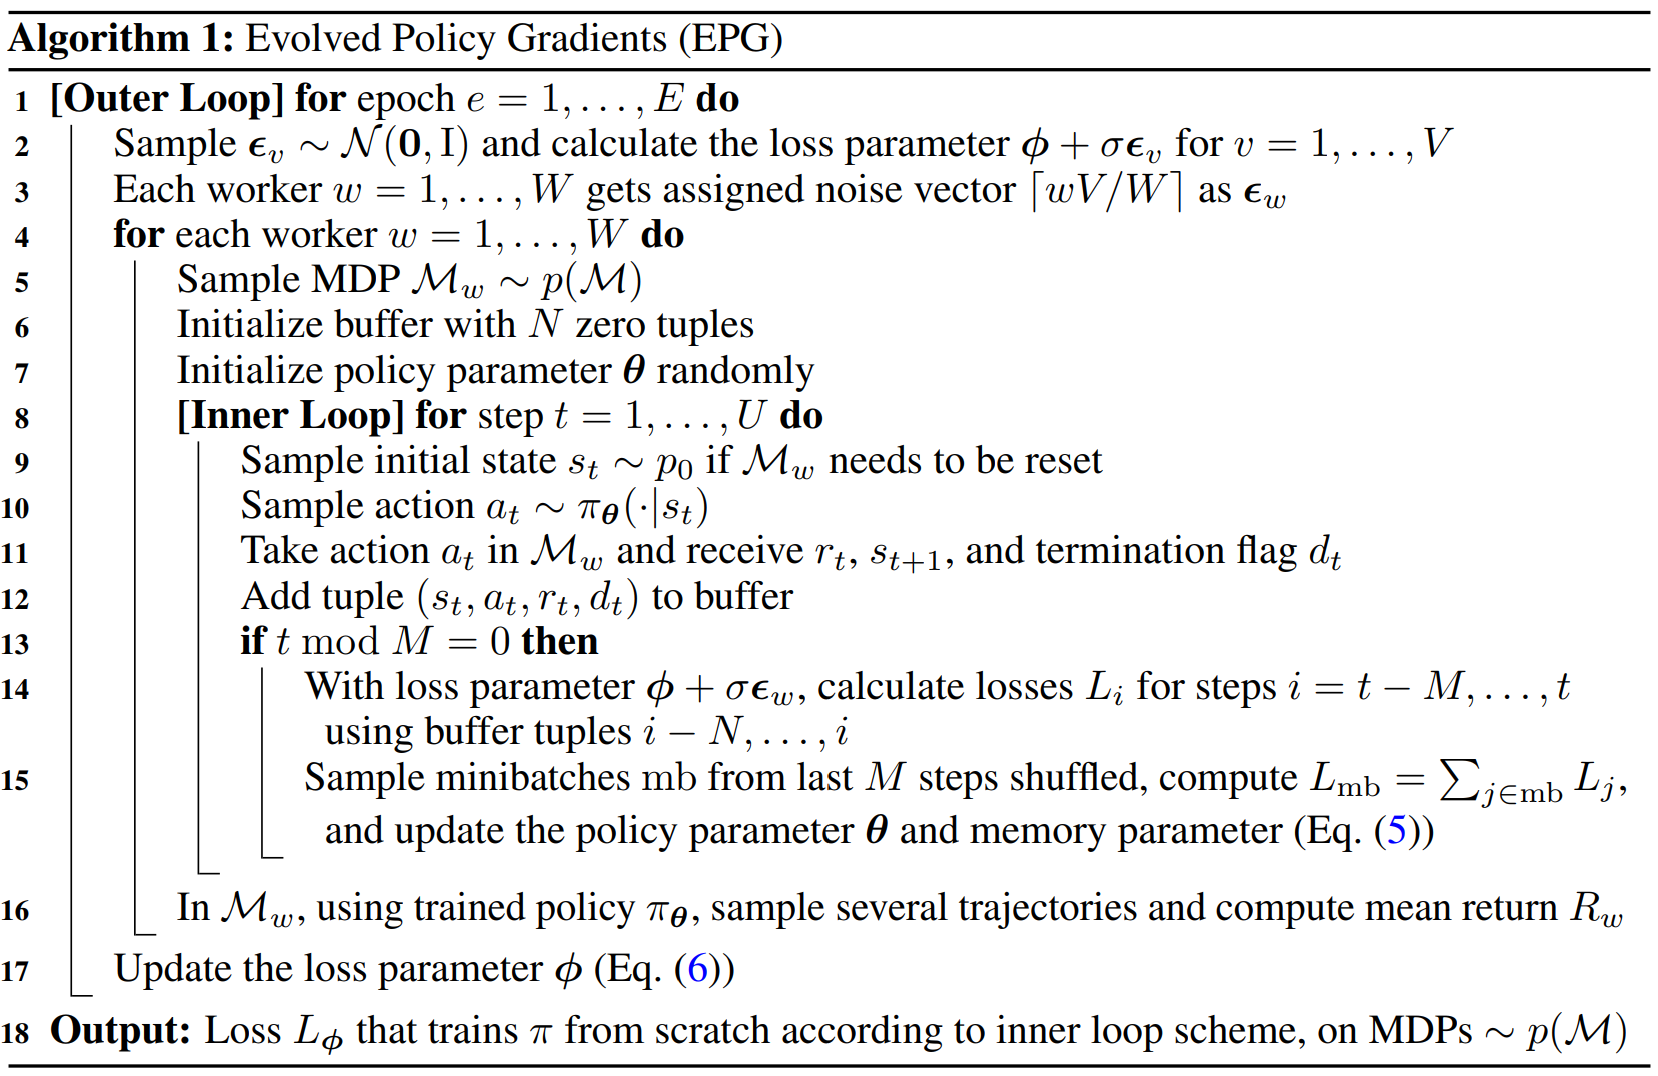
\includegraphics[scale=0.4]{epg.png}
	\centering
	\caption{EPG algorithm.}
	\label{epg}
\end{figure}

\par
Afterwards, the inner loop launches, each worker samples a random MDP from the task distribution $\mathcal{M}_w\thicksim p(\mathcal{M})$ and trains the policy $\pi_\theta$ along with the loss function $L_v$ given from the outer loop, and updates the parameter $\theta$ with learning rate $\delta_{in}$ as follows:

\[\theta\gets\theta - \delta_{in}\cdot\nabla_\theta L_v(\pi_\theta,\tau_{t-M,...,t})\]

\par
At the end of the inner-loop training, the $\textit{w}$-th return $R_w$ is returned by each worker and is aggregated in the outer loop. Then, the parameter $\phi$ of the loss function is updated according to the rule shown below:

\[\phi\gets\phi+\delta_{out}\cdot\frac{1}{V_\sigma}\sum_{v=1}^{V}F(\phi+\sigma\epsilon_v)\epsilon_v\]

where $\delta_{out}$ is the learning rate and $F(\phi+\sigma\epsilon_v) = \frac{R_{(v-1)*W/V+1}+...+R_{v*W/V}}{W/V}$.

\par
The architecture of the loss function can be seen in Fig. \ref{loss-architecture}:
\begin{figure}
	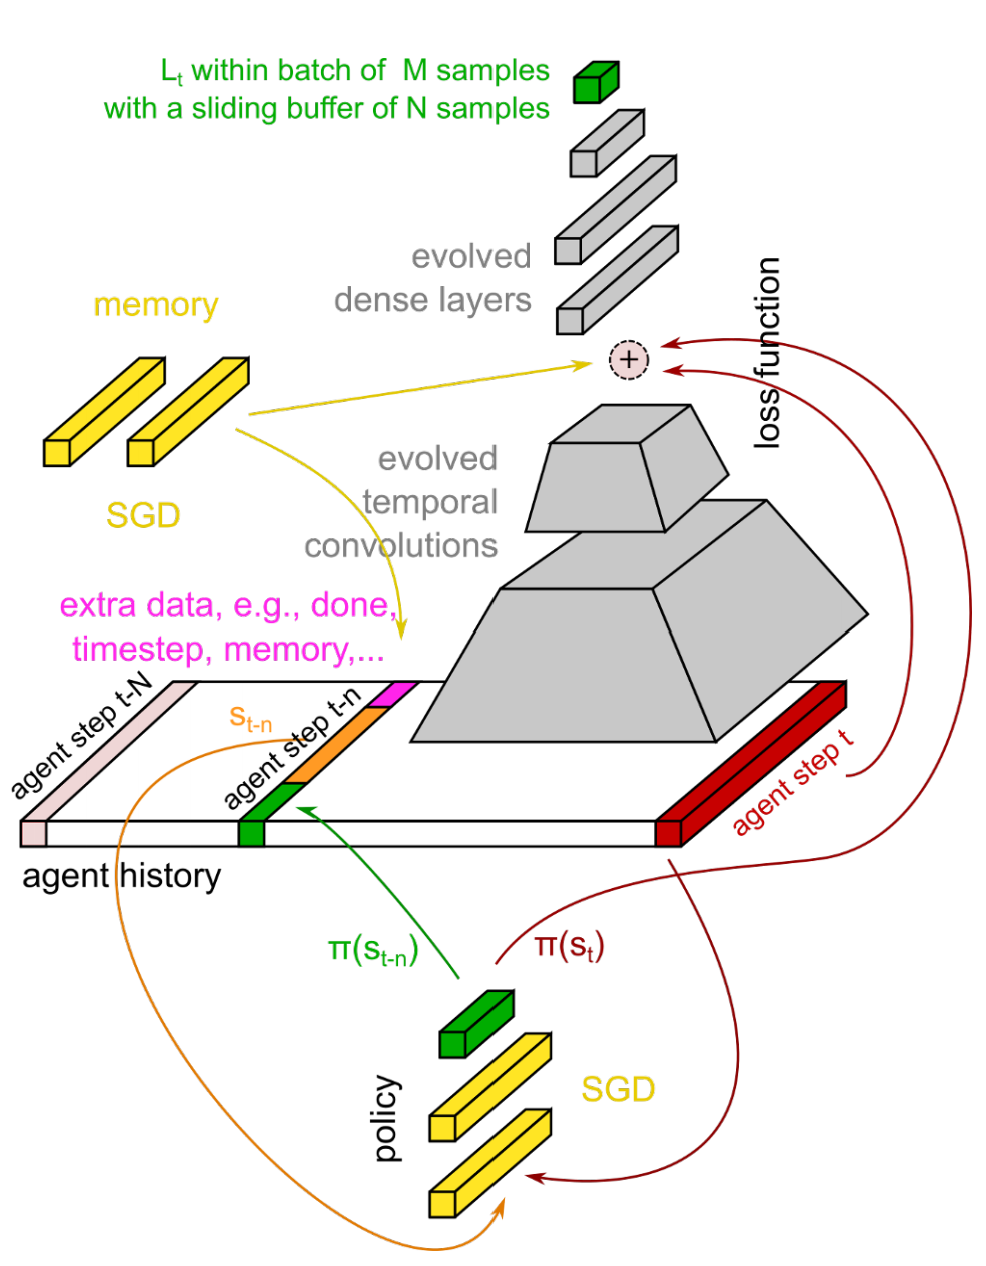
\includegraphics[scale=0.5]{loss-architecture.png}
	\centering
	\caption{Architecture of loss function $L_\phi$.}
	\label{loss-architecture}
\end{figure}

\par
As depicted in the diagram above, the architecture contains a memory unit, which is actually a single-layer neural network accepting constant input vector and is used to store the loss function value, as well as an experience buffer with limited storage, which stores the agent's \textit{N} most recent experience steps, in the form of a list of tuples $(s_t,a_t,r_t,d_t)$ at time step t, where \textit{$d_t$} is the trajectory termination flag. In addition, the architecture consists of temporal convolutional layers which generate a context vector $f_{context}$, and dense layers, which output the loss. The dense layer outputs the loss function \textit{$L_t$} at time step t by taking a batch of \textit{M} sequential samples $\{{s_i,a_i,d_i},mem,f_{context},\pi_\theta(\cdot|s_i)\}^t_{i=t-M}$. To generate the context vector, first, the data samples $\{{s_i,a_i,d_i},mem,\pi_\theta(\cdot|s_i)\}^t_{i=t-N}$ are stack together to form a matrix, second, this matrix is processed by the temporal convolutional layers which outputs the context vector $f_{context}$.

\par
This algorithm is evaluated under several randomized continuous control MuJoCo environments. Fig. \ref{hopper}, \ref{walker}, \ref{reacher} show the evaluation results on RandomHopper, RandomWalker and RandomReacher, which require the agent to identify a randomly sampled environment at test time via exploratory behavior. These diagrams show the learning curves of EPG and the off-the-shelf policy gradient method, PPO, under different settings. We can see that EPG agents learn more quickly and obtain higher returns compared to PPO agents.

\begin{figure}[H]
	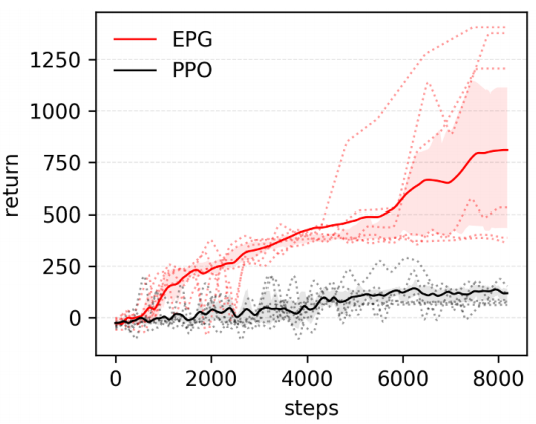
\includegraphics[scale=0.6]{hopper.png}
	\centering
	\caption{RandomHopper testtime training over 128 (policy updates) x64 (update frequency) = 8196 timesteps: PPO vs no-reward EPG.}
	\label{hopper}
\end{figure}
\begin{figure}[H]
	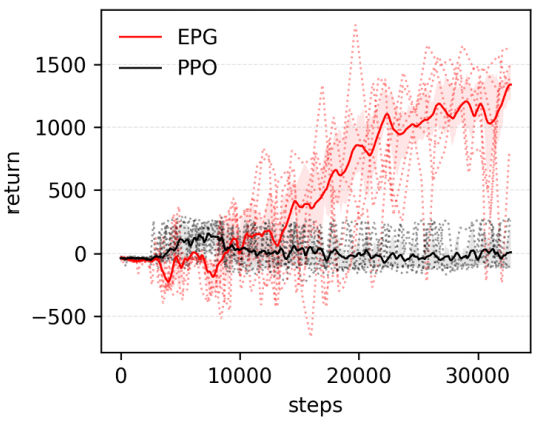
\includegraphics[scale=0.6]{walker.png}
	\centering
	\caption{RandomWalker testtime training over 256 (policy updates) x128 (update frequency) = 32768 timesteps: PPO vs no-reward EPG.}
	\label{walker}
\end{figure}
\begin{figure}[H]
	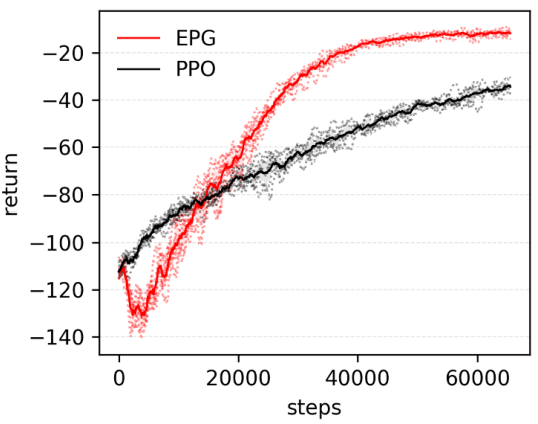
\includegraphics[scale=0.6]{reacher.png}
	\centering
	\caption{RandomReacher testtime training over 512 (policy updates) x128 (update frequency) = 65536 timesteps: PG vs no-reward EPG.}
	\label{reacher}
\end{figure}

\par
Fig. \ref{goal-ant}, \ref{metatrained-direction} and \ref{generalization-direction} show the ability of generalization of EPG. During metatraining, goals are randomly sampled on the positive x-axis (ant walking to the right) and at test time, goals are sampled from the negative x-axis (ant walking to the left). This task is illustrated in Fig. \ref{goal-ant}. Achieving generalization to the left side is not trivial, since it may be easy for a metalearner to overfit to the task metatraining distribution. As shown in Fig. \ref{metatrained-direction}, by training, $RL^2$ converges very fast, while EPG's performance catch up with $RL^2$ after 8192 steps. MAML achieves approximately the same final performance after taking a single SGD step (based on 8000 sampled steps).

\par
But when it comes to the generalization phase, as seen in Fig. \ref{generalization-direction}, the $RL^2$ and MAML algorithm are trapped by overfitting and yield negative result, while EPG trains the agent very quickly to the unseen task.
%We can see from these figures that EPG agents learn more quickly and obtain higher returns compared to PPO agents.

\begin{figure}[H]
	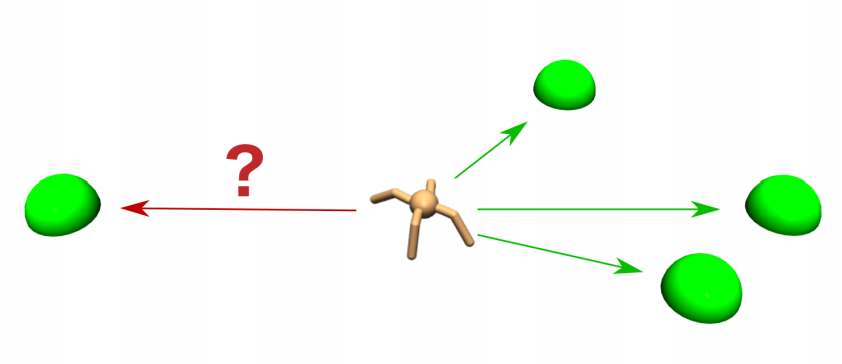
\includegraphics[scale=0.5]{goal-ant-task.png}
	\centering
	\caption{GoalAnt task illustration.}
	\label{goal-ant}
\end{figure}
\begin{figure}[H]
	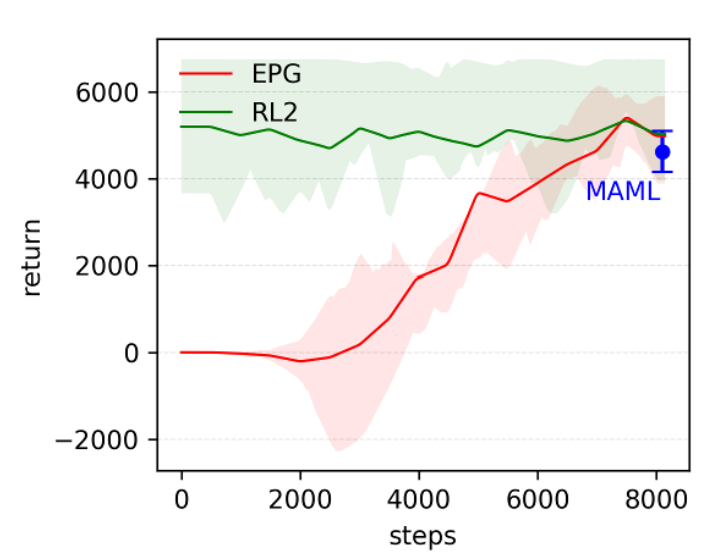
\includegraphics[scale=0.5]{metatrained-direction.png}
	\centering
	\caption{Metatrained direction.}
	\label{metatrained-direction}
\end{figure}
\begin{figure}[H]
	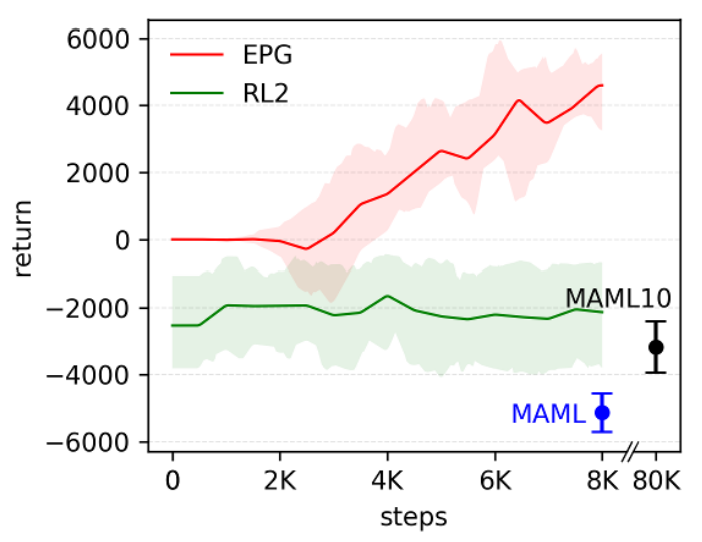
\includegraphics[scale=0.5]{generalization-direction.png}
	\centering
	\caption{Generalization direction.}
	\label{generalization-direction}
\end{figure}